\item Analizar si los siguientes conjuntos son espacios vectoriales sobre $\R$ ($\R$-EV) con las operaciones + y $\cdot$ usuales.
    \begin{enumerate}
        \item Los puntos de una recta de $\R^2$ que pasa por el origen de coordenadas.
            \begin{mdframed}[style=s]
                Los puntos $s$ que pertenecen a dicha recta son de la forma $s=(x,mx)=x(1,m)$ para algún $m$ arbitrario. Con lo cual, el conjunto de puntos lo podemos denotar $S=\overline{\{(1,m)\}}$. En la Figura 1 se observan varios conjuntos de puntos que cumplen con dicha condición. Es claro que $S$ es un subconjunto de $\R^2$ (el cual es un $\R$-espacio vectorial) y se dice que un subconjunto $S$ es un subespacio de $\R^2$ si se cumple:
                \begin{enumerate}
                    \item $\vec{0}\in S$
                    \item si $s_1,s_2 \in S$, luego $s_1+s_2\in S$
                    \item si $s\in S$ y $\lambda \in \mathbb{K} \to \lambda \cdot s \in S$
                \end{enumerate}
                \begin{center}
                    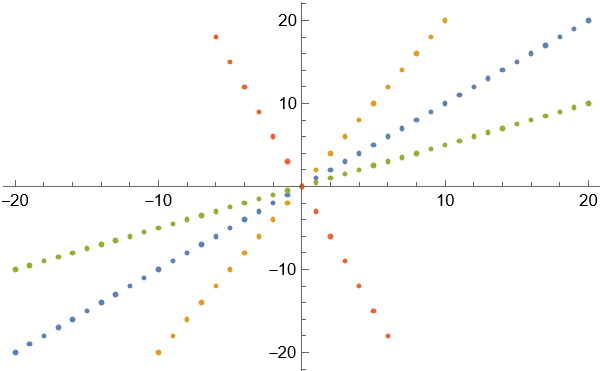
\includegraphics[width=0.4\textwidth]{Ej1a.png}\\
                    Figura 1. Puntos pertenecientes a distintas rectas que incluyen el origen.
                \end{center}
                Además, todo subespacio de un $\R$-espacio vectorial es un $\R$-espacio vectorial.
                \begin{enumerate}
                    \item El $(0,0)=\vec{0}\in S$ ya que la recta pasa por el origen de coordenadas.
                    \item Dados $s_1,s_2\in S, s_1=\alpha(1,m), s_2=\beta(1,m)\to s_1+s_2=\alpha(1,m)+\beta(1,m)=(\alpha + \beta)(1,m)\in S$
                    \item Dados $s\in S, \lambda \in \R, s=\alpha(1,m)\to \lambda s=\lambda\alpha(1,m)=(\lambda\alpha)(1,m)\in S$
                \end{enumerate}
                Como se cumplen las tres condiciones, $S$ es un $\R$-espacio vectorial.
            \end{mdframed}
        \item Las funciones lineales cuya gráfica pertenece a $\R^2$ y contiene al origen de coordenadas.
            \begin{mdframed}[style=s]
                En este caso el conjunto con el que se está tratando es $S=\{f\in \PP_1[x]:f(x)=mx, m\in\R\}$ (Figura 2). Se sabe que el conjunto $\PP_1[x]$ es un espacio vectorial así que como en el caso anterior se verificará que $S$ sea un subespacio.
                \begin{center}
                    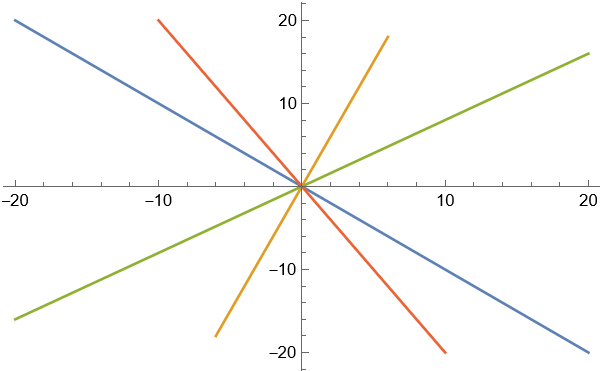
\includegraphics[width=0.4\textwidth]{Ej1b.png}\\
                    Figura 2. Funciones lineales de la forma $f(x)=mx$
                \end{center}
                \begin{enumerate}
                    \item El $0$ de los polinomios es $f(x)=0$, el cual se puede reescribir como $f(x)=0x$, con lo cual pertenece a $S$.
                    \item Dados $f_1,f_2\in S, f_1(x)=m_1x,f_2(x)=m_2x\to (f_1 + f_2)(x)=f_1(x)+f_2(x)=m_1x+m_2x=(m_1+m_2)(x)\in S$
                    \item Dados $f\in S, \lambda \in \R, f(x)=mx\to (\lambda f)(x)=\lambda f(x)=\lambda mx=(\lambda m)(x)\in S$
                \end{enumerate}
                Como se cumplen las tres condiciones, tenemos que S es un espacio vectorial.    
            \end{mdframed}
        \item Los polinomios de grado menor o igual a 3, que tienen el mismo término independiente.
            \begin{mdframed}[style=s]
                En este caso, $S_d=\{p\in \PP_3[x]: p(0)=d, d\in \R\}$. Se puede ver que $S\subset\PP_3[x]$. Sin embargo, hay que tener en cuenta que $S$ está definido según el $d$. Veamos si las 3 condiciones para que un subconjunto sea un subespacio se satisfacen:
                \begin{enumerate}
                    \item Para que el $0$ de los polinomios ($p(x)=0$) forme parte del conjunto, $d=0$, ya que con cualquier otro término independiente este polinomio no estaría incluido.
                    \item Sea $p_1(x)=a_1x^3+b_1x^2+c_1x$ y $p_2(x)=a_2x^3+b_2x^2+c_2x\\\to p_1(x)+p_2(x)=(a_1+a_2)x^3+(b_1+b_2)x^2+(c_1+c_2)x\to p_1+p_2\in S_0$
                    \item Sea $\alpha\in\R$ y $p\in S_0\to (\alpha p)(x)=\alpha ax^3+\alpha bx^2+\alpha cx\in S_0$
                \end{enumerate}
                Con esto se concluye que $S_d$ es un espacio vectorial si $d=0$\vspace{6pt}\\
                ¿Qué pasa si $d\neq 0$?\\
                Lo primero, ya demostrado anteriormente, es que $S_d$ no tendría elemento neutro. Además, supongamos $ p_1,p_2\in S_2$. Al sumarlos y evaluar en $0$ obtengo $(p_1+p_2)(0)=4$, con lo cual la suma no es cerrada. Para visualizar esta situación (ver Figura 3), es conveniente recordar que el término independiente representa la ordenada al origen del polinomio. Es decir, que si dos polinomios tienen la misma ordenada al origen, la suma no necesariamente la mantiene (únicamente si la misma es $0$).
                \begin{center}
                    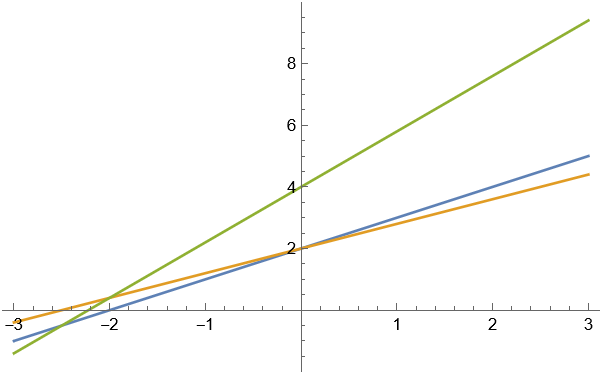
\includegraphics[width=0.4\textwidth]{Ej1c.png}\\
                    Figura 3. Suma de dos polinomios con el mismo término independiente.
                \end{center}
                Otra cuestión a considerar es el producto por escalar. Supongamos que tengo $p(x)=x+1\in S_1\to(2 p)(x)=2x+2\notin S_1$, por lo tanto, tampoco es cerrado bajo el producto por escalar.  
            \end{mdframed}
        \item Las matrices de $\R^{2\times2}$ cuya diagonal principal es nula.
            \begin{mdframed}[style=s]
                Estas matrices son de la forma 
                \begin{tightcenter}
                    $A=\begin{pmatrix}
                        0&a\\
                        b&0
                    \end{pmatrix}$
                \end{tightcenter}
                Con lo cual el conjunto en cuestión es 
                \begin{tightcenter}
                    $S=\overline{\left\{\begin{pmatrix}
                        0&1\\
                        0&0
                    \end{pmatrix}\begin{pmatrix}
                        0&0\\
                        1&0
                    \end{pmatrix}\right\}}$    
                \end{tightcenter}
                Se sabe que $\R^{2\times2}$ es un espacio vectorial. Con lo cual si se comprueban las 3 condiciones presentadas anteriormente, el conjunto de las matrices que respetan la forma de $A$ será un espacio vectorial.
                \begin{enumerate}
                    \item $\begin{pmatrix}
                            0&0\\
                            0&0
                        \end{pmatrix}\in S$ ya que $\begin{pmatrix}
                            0&0\\
                            0&0
                        \end{pmatrix}=0\cdot\begin{pmatrix}
                            0&1\\
                            0&0
                        \end{pmatrix}+0\cdot\begin{pmatrix}
                            0&0\\
                            1&0
                        \end{pmatrix}$
                    \item Sea $\alpha\in\R$ y $A\in S\to \alpha A=\alpha \begin{pmatrix}
                            0&a\\
                            b&0
                        \end{pmatrix}=\begin{pmatrix}
                            0&\alpha a\\
                            \alpha b&0
                        \end{pmatrix}\in S$
                    \item Sean $A_1,A_2\in S\to A_1+A_2=\begin{pmatrix}
                            0&a_1\\
                            b_1&0
                        \end{pmatrix}+\begin{pmatrix}
                            0&a_2\\
                            b_2&0
                        \end{pmatrix}=\begin{pmatrix}
                            0&a_1+a_2\\
                            b_1+b_2&0
                        \end{pmatrix}\in S$
                \end{enumerate}
                Por lo tanto, $S$ es un espacio vectorial.
            \end{mdframed}
        \item Las matrices de $\R^{3\times3}$ inversibles.
            \begin{mdframed}[style=s]
                Para que una matriz $A$ sea inversible, debe existir una segunda matriz $B$ tal que: $AB=BA=I$.
                \begin{enumerate}
                    \item La matriz nula no es inversible, ya que $0\cdot B=0\quad\forall B\in\R^{3\times3}$
                \end{enumerate}
                Por lo tanto, estas matrices no son un espacio vectorial.
            \end{mdframed}
    \end{enumerate}